%----------------------------------------------------------------------------------------
%	SLIDE 2.
%----------------------------------------------------------------------------------------
\begin{frame}
\frametitle{Absolute limits}

\begin{itemize}
	\item General relativity: the Einstein's equations should hold for the stellar structure
	\item Le Chatelier's principle: for small distortions, an NS in equilibrium will bounce back to an equilibrium ($\mathrm{d}p / \mathrm{d} \rho \geq 0$)
	\item Causality: Speed of sound in the NS should not be larger than the speed of light ($\sqrt{\mathrm{d}p / \mathrm{d} \epsilon} \leq 1$)
\end{itemize}
\begin{figure}
	\centering
	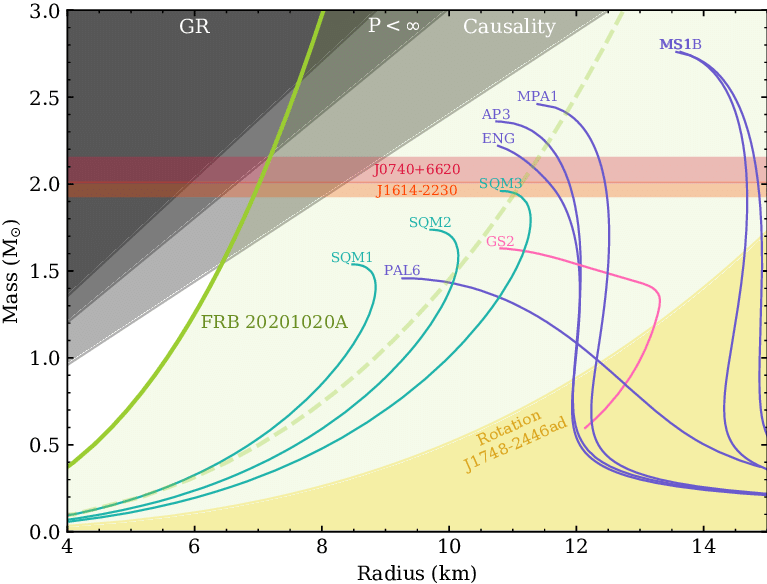
\includegraphics[width=0.5\linewidth]{./images/ns-limiting-factors.png}
\end{figure}

\end{frame}